%----------------------------------------------------------------------------------------
%	PACKAGES AND THEMES
%----------------------------------------------------------------------------------------

\documentclass{beamer}

\mode<presentation> {
\usetheme{Madrid}
}

\usepackage{graphicx}
\usepackage{booktabs}
\usepackage{polski}
\usepackage[polish]{babel}
\usepackage[utf8]{inputenc}
\usepackage[T1]{fontenc}
\usepackage[utf8]{luainputenc}
\usepackage{pgfgantt}
\usepackage{caption}
\DeclareCaptionFormat{citation}{%
   \ifx\captioncitation\relax\relax\else
     \captioncitation\par
   \fi
   #1#2#3\par}
\newcommand*\setcaptioncitation[1]{\def\captioncitation{\tiny{\textit{Źródło:}~#1}\medskip}\normalsize}
\let\captioncitation\relax
\captionsetup{format=citation,justification=centering}

%----------------------------------------------------------------------------------------
%	TITLE PAGE
%----------------------------------------------------------------------------------------

\title[Seminarium Dyplomowe Inżynierskie]{Integracja części manipulacyjnej i bazy mobilnej robota Velma na potrzeby symulacji}

\author{Jakub Sikora} 
\institute[]
{
Zakład Sterowania Systemów \\
Instytut Automatyki i Informatyki Stosowanej \\
\medskip
Promotor: dr inż. Tomasz Winiarski
}
\date{25 października 2019}

\AtBeginSection[]
{
    \begin{frame}[plain, noframenumbering]
        \frametitle{Agenda}
        \tableofcontents[currentsection]
    \end{frame}
}

\begin{document}

\begin{frame}
\titlepage
\end{frame}

\begin{frame}
\frametitle{Agenda}
\tableofcontents
\end{frame}

%----------------------------------------------------------------------------------------
%	PRESENTATION SLIDES
%----------------------------------------------------------------------------------------

\section{Cele pracy} 

%------------------------------------------------

\begin{frame}
\frametitle{Cele pracy (I)}
\begin{block}{Integracja symulatorów}
Połączenie istniejącego symulatora korpusu robota Velma z symulatorem holonomicznej bazy mobilnej.
\end{block}
\end{frame}

%------------------------------------------------

\begin{frame}
\frametitle{Cele pracy (II)}
\begin{block}{System sterowania}
Zaprojektowanie i przetestowanie systemu sterowania zintegrowanym systemem robotycznym przed uruchomieniem go na rzeczywistym sprzęcie.
\end{block}
\end{frame}

%------------------------------------------------

\section{Tematyka pracy}
%------------------------------------------------

\begin{frame}
\frametitle{Table}
\begin{table}
\begin{tabular}{l l l}
\toprule
\textbf{Treatments} & \textbf{Response 1} & \textbf{Response 2}\\
\midrule
Treatment 1 & 0.0003262 & 0.562 \\
Treatment 2 & 0.0015681 & 0.910 \\
Treatment 3 & 0.0009271 & 0.296 \\
\bottomrule
\end{tabular}
\caption{Table caption}
\end{table}
\end{frame}

%------------------------------------------------

\begin{frame}
\frametitle{Theorem}
\begin{theorem}[Mass--energy equivalence]
$E = mc^2$
\end{theorem}
\end{frame}

%------------------------------------------------

\begin{frame}[fragile] % Need to use the fragile option when verbatim is used in the slide
\frametitle{Verbatim}
\begin{example}[Theorem Slide Code]
\begin{verbatim}
\begin{frame}
\frametitle{Theorem}
\begin{theorem}[Mass--energy equivalence]
$E = mc^2$
\end{theorem}
\end{frame}\end{verbatim}
\end{example}
\end{frame}

%------------------------------------------------

\begin{frame}
\frametitle{Figure}
Uncomment the code on this slide to include your own image from the same directory as the template .TeX file.
%\begin{figure}
%\includegraphics[width=0.8\linewidth]{test}
%\end{figure}
\end{frame}

%------------------------------------------------

\begin{frame}[fragile] % Need to use the fragile option when verbatim is used in the slide
\frametitle{Citation}
An example of the \verb|\cite| command to cite within the presentation:\\~

This statement requires citation \cite{p1}.
\end{frame}


\section{Przegląd istniejących rozwiązań}

%------------------------------------------------

\begin{frame}
\frametitle{Robot Velma}
\begin{figure}
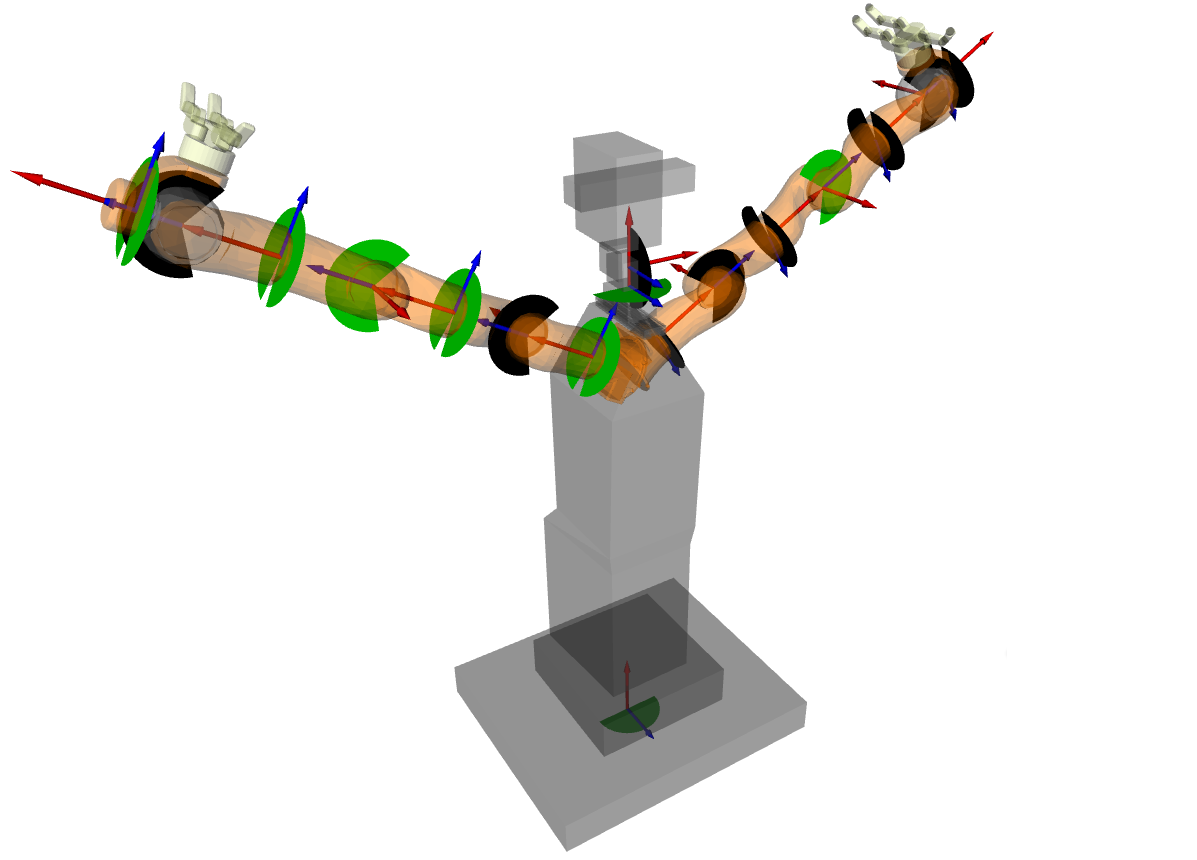
\includegraphics[scale=0.22]{./images/velma_joints.png}
\setcaptioncitation{\texttt{https://rcprg-ros-pkg.github.io/velma\_docs/2017/10/13/01/01\_{}introduction\_{}02\_{}velma\_{}robot/}}
\caption{Wizualizacja robota Velma z zaznaczonymi stopniami swobody \cite{docsVelma}}
\end{figure}
\end{frame}

%------------------------------------------------

\begin{frame}
\frametitle{Robot Velma}
\begin{figure}
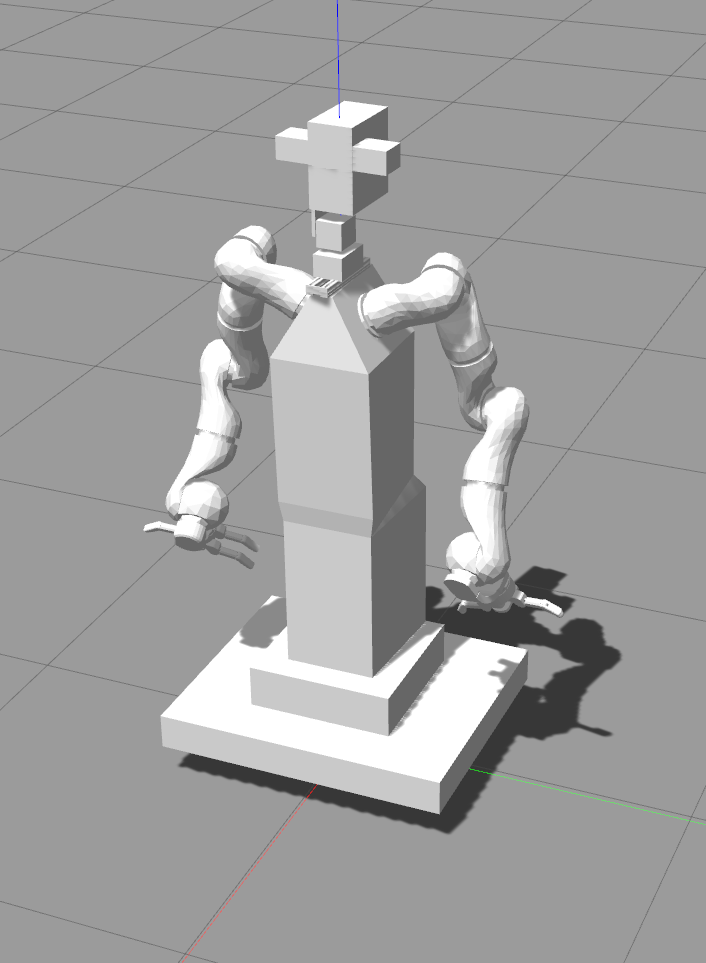
\includegraphics[scale=0.20]{./images/velma_gz_cropped.png}
\caption{Robot Velma w symulatorze Gazebo}
\end{figure}
\end{frame}

%------------------------------------------------

\begin{frame}
\frametitle{Robot Velma}
Robot Velma składa się z \cite{docsVelma}:  
\begin{itemize}
	\item obrotowego korpusu
	\item dwóch manipulatorów KUKA LWR
	\item dwóch chwytaków BarrettHand
	\item szyi o dwóch stopniach swobody
	\item kamery Kinect XBOX 360
\end{itemize}
\end{frame}

%------------------------------------------------

\begin{frame}
\frametitle{Struktura symulatora}

\end{frame}

%------------------------------------------------

\begin{frame}
\frametitle{Robot Velmobil}
\begin{figure}
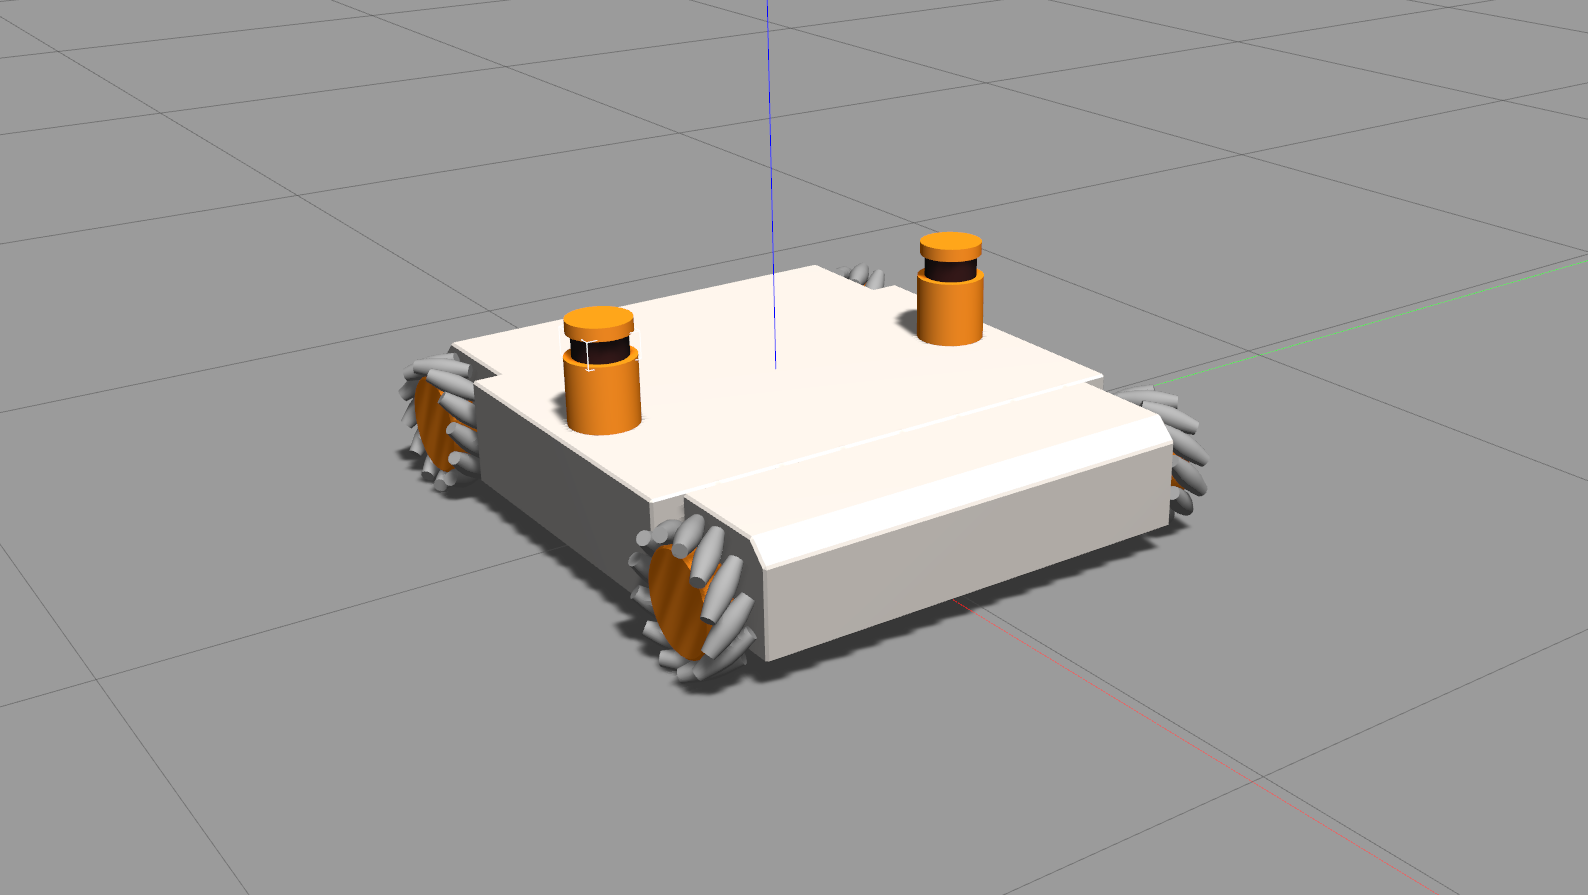
\includegraphics[scale=0.20]{./images/omnivelma_gz.png}
\caption{Baza mobilna robota w symulatorze Gazebo}
\end{figure}
\end{frame}

%------------------------------------------------

\begin{frame}
\frametitle{Robot Velmobil}
Robot Velmobil posiada \cite{docsVelma}:  
\begin{itemize}
	\item 4 koła szwedzkie
	\item dwa skanery laserowe LIDAR
	\item jednostkę inercyjną
	\item enkodery % jakie enkodery
\end{itemize}
\end{frame}

%------------------------------------------------

\begin{frame}
\frametitle{Struktura symulatora}

\end{frame}
\section{Sformułowanie zadań pracy}

%------------------------------------------------

\begin{frame}
	\frametitle{Przystosowanie symulatorów do pracy}
	\begin{itemize}
		\item Uruchomienie symulatora korpusu
		\item Uruchomienie symulatora bazy mobilnej
		\item Przystosowanie komponentów do pracy z najnowszą wersją Gazebo 
	\end{itemize}
\end{frame}

%------------------------------------------------

\begin{frame}
	\frametitle{Stworzenie zintegrowanego modelu}
	\begin{itemize}
		\item Unifikacja modelu korpusu oraz bazy mobilnej
		\item Stworzenie adaptera łączącego oba komponenty 
	\end{itemize}
\end{frame}

%------------------------------------------------

\begin{frame}
	\frametitle{Komponent sterujący w ROS}
	\begin{itemize}
		\item Stworzenie węzła ROS odpowiedzialnego za sterowanie systemem
		\item Wykorzystanie wcześniej stworzonego adaptera
		\item Realizacja zadania testowego
	\end{itemize}
\end{frame}

%------------------------------------------------

\begin{frame}
	\frametitle{Przygotowanie dokumentacji systemu}
	\begin{itemize}
		\item Przygotowanie dokumentacji dla przyszłych użytkowników platformy
		\item Przygotowanie diagramów struktur i zachowań w SysML
	\end{itemize}
\end{frame}

%------------------------------------------------

\section{Wyniki pracy}

%------------------------------------------------

\begin{frame}
    \frametitle{Uruchomienie symulatorów}
    \begin{figure}
        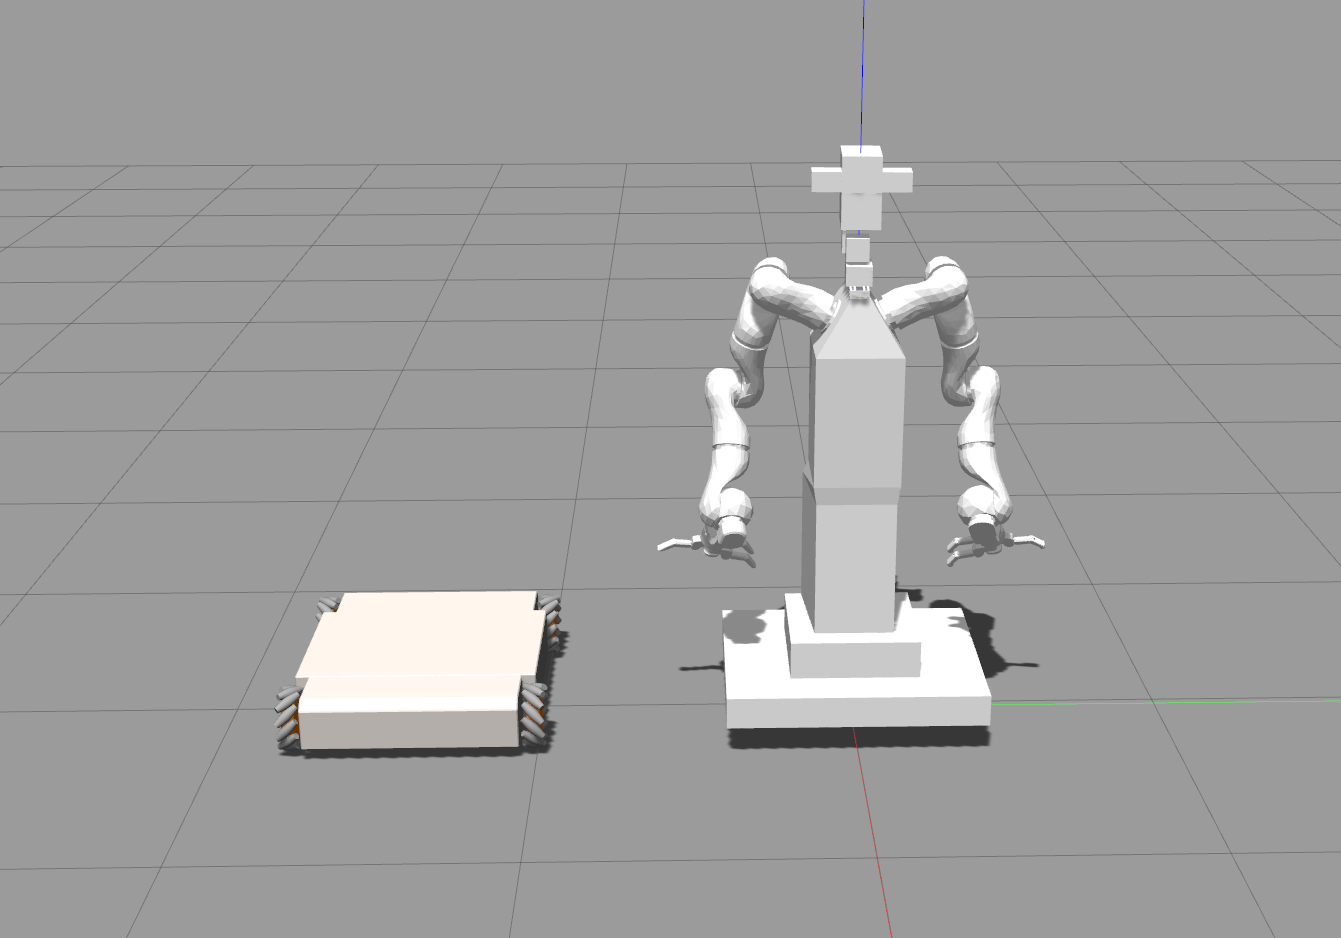
\includegraphics[scale=0.20]{./images/velma+omnivelma_cropped.png}
        \caption{Modele korpusu i bazy mobilnej w jednym świecie symulacji}
    \end{figure}
\end{frame}

%------------------------------------------------

\begin{frame}
    \frametitle{Proste zadanie manipulacji}
    \begin{figure}
        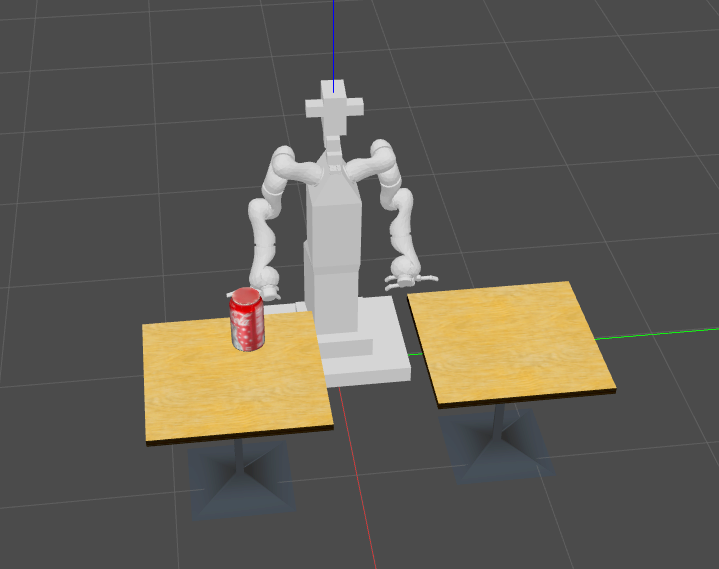
\includegraphics[scale=0.35]{./images/velma_stero_task.png}
        \caption{Zadanie przenoszenia puszki ze stolika na stolik}
    \end{figure}
\end{frame}

%------------------------------------------------

\begin{frame}
	\frametitle{Projekt koncepcyjny systemu}
	\bigskip
	\begin{figure}
        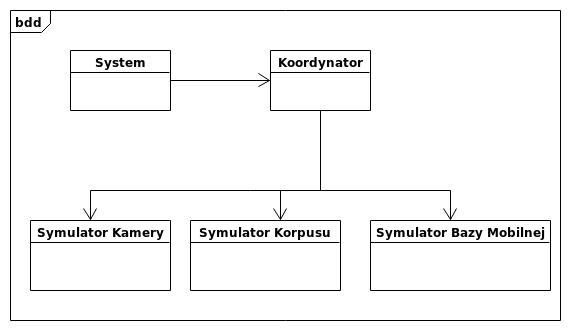
\includegraphics[scale=0.5]{./images/example_bdd.png}
        \caption{Poglądowa struktura systemu w SySML}
    \end{figure}
\end{frame}

%------------------------------------------------
\section{Plan prac na bieżący semestr}

\begin{frame}
	\frametitle{Zadania}
	\begin{block}{Integracja modeli}
	Stworzyć jednolity system uruchamiania obu komponentów w symulatorze
	Gazebo, tak aby korpus znalazł się na bazie mobilnej.
	\end{block}
	\medskip
	\begin{block}{Implementacja sterownika}
	Na podstawie wcześniejszego projektu systemu, zaimplementować 
	sterownik jako węzeł ROS. Założyć że komponenty poruszają się 
	niezależnie od siebie.
	\end{block}
\end{frame}


%------------------------------------------------

\begin{frame}
	\frametitle{Harmonogram prac}
	\centering
	\begin{ganttchart}[hgrid, vgrid]{1}{18}
		\gantttitle{Październik}{5} 
		\gantttitle{Listopad}{4}
		\gantttitle{Grudzień}{5} 
		\gantttitle{Styczeń}{4} \ganttnewline
		\ganttbar{Specyfikacja}{1}{3} \ganttnewline
		\ganttbar{Model}{1}{6} \ganttnewline
		\ganttbar{Sterownik}{7}{11} \ganttnewline
		\ganttbar{Praca inż.}{3}{6}  \ganttbar{}{12}{18} \ganttnewline
		\ganttmilestone{Seminarium}{4} \ganttmilestone{}{11} 
		\ganttlink{elem1}{elem2}
		\ganttlink{elem2}{elem4}
		\ganttlink{elem0}{elem2}
		\ganttlink{elem0}{elem3}
		\end{ganttchart}
\end{frame}

%------------------------------------------------
\section{Podsumowanie}


% dodatkowe założenia

\begin{frame}
    \frametitle{Założenia ruchu}
\end{frame}

% perspektywy rozwoju

\begin{frame}
    \frametitle{Implementacja w sprzęcie}
\end{frame}
%------------------------------------------------

\begin{frame}[plain]
\addtocounter{framenumber}{-1}
\frametitle{Bibliografia}
\footnotesize{
\begin{thebibliography}{99} % Beamer does not support BibTeX so references must be inserted manually as below
\bibitem[1]{docsVelma} D. Seredyński
\newblock Documentation of control system of WUT Velma Robot, 2017.
\newblock \url{https://rcprg-ros-pkg.github.io/velma\_docs/}.

\bibitem[2]{walas} P. Walas
\newblock Nawigacja robota mobilnego w bezpośrednim otoczeniu człowieka
\newblock \emph{Praca dyplomowa inżynierska}, Promotor: dr hab. inż. Wojciech Szynkiewicz, 2018.

\bibitem[3]{bezpieczenstwo} T.Winiarski
\newblock Wybrane aspekty bezpieczeństwa w badaniach robotów usługowych
\newblock \emph{Politechnika Warszawska}, materiały do Sterowania i Symulacji Robotów, 2018.

\bibitem[4]{sterowanie} T. Winiarski, C. Zieliński
\newblock Podstawy sterowania siłowego robotów
\newblock{Pomiary Automatyka Robotyka}, 6/2008, strony 5-10.

\end{thebibliography}
}
\end{frame}

%------------------------------------------------

\begin{frame}[plain]
\addtocounter{framenumber}{-1}
\Huge{\centerline{Dziękuje za uwagę}}
\end{frame}

%% dodatkowe
\addtocounter{framenumber}{-1}
\begin{frame}[plain]
    \frametitle{Komunikacja w ROS}
    Węzły w ROS mogą komunikować się ze sobą za pomocą:
    \begin{itemize}
        \item \textbf{tematów} - wykorzystywane do publikowania danych ciągłych takich jak dane z czujnika, stan stawu itp.
        \item \textbf{serwisów} - wykorzystywane do wywoływania zdalnych krótkich procedur, gdzie wymagany jest tylko końcowy wynik
        \item \textbf{akcji} - wykorzystywane do dyskretnych procesów, w których ważna jest informacja zwrotna w trakcie wykonywania  
    \end{itemize}   
\end{frame}

\end{document} 